%%% !TEX TS-program = XeLaTeX
\documentclass[oneside,bsc,12pt]{AUTthesis}

\input{commands}
\setlength{\headheight}{15pt}

\begin{document}
\baselineskip=.75cm
\linespread{1.75}
%% -!TEX root = AUTthesis.tex
\faculty{دانشکده ریاضی و علوم کامپیوتر}
\department{علوم کامپیوتر}
\fatitle{ساخت خودکار گراف دانش از متن غیرساختاریافته با مدل‌های زبانی}
\firstsupervisor{دکتر مهدی قطعی}
\secondsupervisor{دکتر بهنام یوسفی مهر}
\name{مصطفی}
\surname{رستگار}
\thesisdate{شهریور 1405}

\fa-abstract{
بخش بزرگی از دانش هر سازمانی در متن آزاد پراکنده است و هیچ‌جا به شکلی ذخیره نشده که بشود از آن پرس‌وجو گرفت. این پژوهش سامانه‌ای می‌سازد که از متن غیرساختاریافته سه‌تایی‌های «موجودیت، رابطه، موجودیت» را بیرون می‌کشد و آن‌ها را در یک گراف دانش قابل پرس‌وجو می‌نشاند. آنچه این سامانه را از یک فراخوانی ساده مدل زبانی جدا می‌کند سه تصمیم است: هستان‌شناسی مقیّد که هر سه‌تایی خارج از فهرست ترکیب‌های مجاز را رد می‌کند، الزام شاهد که هر یال را به جمله منبعش گره می‌زند، و خط لوله‌ای که هرچند بار اجرا شود داده تکراری نمی‌سازد.
\\
سامانه روی بنچمارک استاندارد \lr{Re-DocRED} ارزیابی شد. در شش تکرار، مقدار $F_1$ از $16.88$ به $29.66$ رسید، در حالی که خط مبنای منتشرشده با \lr{GPT-3.5} روی همین داده $9.74$ است. سپس همان پیکربندی روی کل $500$ سند بخش \lr{Dev} اجرا شد و $28.64$ گرفت. در مرحله سوم، داده به پیکره کامل \lr{DocRED} با $106{,}924$ سند و $1.56$ میلیون سه‌تایی برچسب‌خورده گسترش یافت و خط لوله برای این مقیاس بازنویسی شد: استخراج هم‌زمان، ازسرگیری بدون دوباره‌کاری، ارزیاب جریانی و بارگذار دسته‌ای.
\\
با تغییر مدل زبانی، فشرده کردن قالب پاسخ و گرفتن اشتراک دو گذر به‌جای اجتماعشان، مقدار $F_1$ روی $998$ سند بخش \lr{Dev} به $36.25$ و روی $3{,}053$ سند بخش \lr{Train} برچسب‌خورده، که در تنظیم پرامپت نقشی نداشت، به $36.33$ رسید. نزدیکی این دو عدد نشان می‌دهد سامانه روی بخش \lr{Dev} بیش‌برازش نشده است. یک مجموعه پیش‌بینی ثابت روی $498$ سند مشترک، با برچسب اصلی دقت $40.20$ و با برچسب بازبینی‌شده دقت $66.42$ می‌گیرد؛ این اختلاف، اندازه‌گیری مستقیم مسئله منفی کاذب در برچسب‌های اصلی \lr{DocRED} است. گراف نهایی از $16{,}536$ سند ساخته شد و $111{,}912$ موجودیت، $253{,}007$ رابطه و $278{,}632$ گره شاهد دارد. در پایان، همان سامانه بدون تغییر معماری روی اسناد فارسی شهرداری اجرا شد و تنها چیزی که عوض شد یک فایل هستان‌شناسی بود.
}

\keywords{گراف دانش، استخراج رابطه در سطح سند، مدل زبانی بزرگ، هستان‌شناسی مقیّد، مهار توهم، \lr{DocRED}}

\AUTtitle
\vspace*{7cm}
\thispagestyle{empty}
\begin{center}

\includegraphics[height=5cm,width=12cm]{Images/besm.jpg}
\end{center}

\input{taid}
\input{fa_abstract}
\pagenumbering{alph}
\input{TOC-TOF-LOT}
%%%%%%%%%%%%%

{\centering\LARGE\textbf{فهرست نمادها}\par}%

\pagenumbering{alph}
\setcounter{page}{\thesavepage}
\vspace*{1cm}

\pagestyle{style3}
\symb{\text{ نماد}}{مفهوم}
\\
%مقادیر بالا را تغییر ندهید
%%%%%%%%%%%%%%%%%%%%%%%%%%%%%%%%%%%%%%%%%%%%%%%%%%%%%%%%%
\symb{(h, r, t)}{
سه‌تایی استخراج‌شده: موجودیت مبدأ، رابطه، موجودیت مقصد
}
\symb{P}{
دقت؛ نسبت سه‌تایی‌های درست به کل سه‌تایی‌های پیش‌بینی‌شده
}
\symb{R}{
بازخوانی؛ نسبت سه‌تایی‌های درست به کل سه‌تایی‌های طلایی
}
\symb{F_1}{
میانگین هماهنگ دقت و بازخوانی
}
\symb{\mathrm{Ign}\,F_1}{
مقدار $F_1$ پس از حذف حقیقت‌هایی که در بخش \lr{Train} هم دیده شده‌اند
}
\symb{\mathcal{O}}{
هستان‌شناسی؛ مجموعه ترکیب‌های مجاز نوع فاعل، رابطه و نوع مفعول
}
\symb{|\mathcal{O}|}{
تعداد ترکیب‌های مجاز؛ برای \lr{Re-DocRED} برابر $654$
}
\symb{e}{
متن شاهد؛ عین جمله منبعی که یک رابطه از آن استخراج شده است
}
\symb{A \cap B}{
اشتراک دو گذر مستقل استخراج؛ سه‌تایی‌هایی که هر دو گذر یافته‌اند
}
\symb{A \cup B}{
اجتماع دو گذر مستقل استخراج
}
\symb{R_1, R_2, R_3}{
سه قاعده لایه بستار: وارون، تراگذری و زنجیره کشور
}


\pagenumbering{arabic}
\pagestyle{style1}

\chapter{مقدمه}
\label{ch:intro}

بخش بزرگی از دانش هر سازمانی جایی ذخیره نشده که بشود از آن پرس‌وجو گرفت و در متن آزاد پراکنده است. برای پاسخ به پرسشی که در نگاه اول ساده می‌آید، مثلاً اینکه مجری فلان پروژه چه شرکتی بوده یا فلان شخص تابع کدام کشور است، باید ده‌ها سند را دستی خواند و کنار هم گذاشت.

گراف دانش راه‌حل شناخته‌شده این وضعیت است: متن به گره و یال تبدیل می‌شود و پرسش، به‌جای خواندن، با یک پرس‌وجو پاسخ می‌گیرد. مسئله این است که ساختن خود گراف از متن، کار ساده‌ای نیست.

\section{بیان مسئله}
\label{sec:problem}

آنچه در این پژوهش دنبال شد، استخراج رابطه در سطح سند\LTRfootnote{Document-level Relation Extraction} است. ورودی یک متن چندجمله‌ای است و خروجی مجموعه‌ای از سه‌تایی‌ها که هرکدام به جمله منبع خود گره خورده‌اند. دو چیز کار را سخت می‌کند.

اولی اینکه رابطه معمولاً در یک جمله جمع نشده و مدل باید چند جمله را دنبال کند و از زنجیره هم‌مرجعی رد شود. دومی که به نظر ما جدی‌تر است، این است که مدل زبانی رابطه نادرست می‌سازد. برای یک گراف دانش این خطا از خطای معمول بدتر است، چون یال غلط یک بار وارد می‌شود و بعد برای همیشه در پایگاه‌داده می‌ماند و به پرسش‌های بعدی هم سرایت می‌کند.

\section{مشارکت‌های این کار}
\label{sec:contributions}

ایده محوری این است که به مدل زبانی اعتماد نکنیم و خروجی‌اش را از چند صافی رد کنیم. پنج جزء زیر روی هم این کار را انجام می‌دهند.

\subsection{هستان‌شناسی مقیّد}
\label{sec:c-ontology}

سه‌تایی تنها وقتی پذیرفته می‌شود که ترکیب «نوع فاعل، رابطه، نوع مفعول» آن در فهرست مجاز باشد و هر چیز دیگری بی‌چون‌وچرا کنار گذاشته می‌شود. این صافی در اجرا روی \lr{Re-DocRED} یک‌پنجم خروجی مدل، یعنی $20.3\%$، را رد کرد و همان‌طور که در بخش \ref{sec:supervision} نشان می‌دهیم، بهایی که بابتش پرداختیم تنها $0.21\%$ از بازخوانی بود.

\subsection{شاهد اجباری}
\label{sec:c-evidence}

هر یال باید عین جمله منبع را با خود حمل کند و یال بی‌شاهد اصلاً وارد گراف نمی‌شود. حاصلش این است که هیچ ادعایی در گراف نمی‌ماند که نشود آن را تا متن اصلی دنبال کرد.

\subsection{لایه بستار قاعده‌محور}
\label{sec:c-closure}

مدل زبانی آنچه را می‌گوید که در جمله نوشته شده، اما گراف دانش باید آنچه را هم نگه دارد که از خود گراف نتیجه می‌شود. سه قاعده روی گراف اجرا می‌شوند و حقیقت‌های تازه می‌سازند. نکته طراحی اینجاست که هر حقیقت استنتاجی شاهد مقدمه‌های خود را به ارث می‌برد، پس قانون بند قبل زیر پا گذاشته نمی‌شود.

\subsection{خط لوله تکرارپذیر}
\label{sec:c-idempotent}

سند تازه اضافه کنید و دوباره اجرا کنید؛ نه سند تکراری ساخته می‌شود، نه قطعه، نه سه‌تایی، نه گره و نه یال. این را با کلید پایدار \lr{entity\_key} برای گره‌ها، \lr{fact\_id} مبتنی بر \lr{sha1} برای یال‌ها و کش در سطح \lr{chunk\_sha} به دست آوردیم.

\subsection{ورودی چندقالبی}
\label{sec:c-input}

علاوه بر \lr{PDF} و \lr{DOCX} و \lr{TXT}، تصویر هم پذیرفته می‌شود و با مدل بینایی رونویسی می‌گردد.

\section{ساختار گزارش}
\label{sec:structure}

فصل \ref{ch:related} کارهای پیشین و مبانی لازم را مرور می‌کند. فصل \ref{ch:method} معماری سامانه، هستان‌شناسی، لایه بستار و مهندسی لازم برای مقیاس صدهزار سندی را شرح می‌دهد. فصل \ref{ch:dataset} داده و آرایش آزمایش و معیارها را معرفی می‌کند و توضیح می‌دهد سامانه دقیقاً از چه نظارتی استفاده می‌کند. فصل \ref{ch:results} نتایج سه مرحله کار و تحلیل خطا را می‌آورد. فصل \ref{ch:casestudy} همان سامانه را روی اسناد فارسی اجرا می‌کند و فصل \ref{ch:conclusion} محدودیت‌ها و جمع‌بندی را می‌گوید.

\chapter{کارهای پیشین و مبانی نظری}
\label{ch:related}

\section{چهار رویکرد موجود}
\label{sec:approaches}

جدول \ref{tab:related} چهار خانواده روش را کنار هم می‌گذارد. کار حاضر در دسته سوم است، ولی خطای آن را با یک لایه نمادین مهار می‌کند. این ترکیب در ادبیات ساخت گراف دانش عصبی\lr{--}نمادین\LTRfootnote{Neuro-symbolic Knowledge Graph Construction} نامیده می‌شود.

\begin{table}[ht]
\centering
\caption{مقایسه چهار رویکرد موجود برای ساخت گراف دانش از متن.}
\label{tab:related}
\small
\begin{tabular}{|p{3.5cm}|p{4.3cm}|p{5.9cm}|}
\hline
\rg رویکرد & \rg نقطه قوت & \rg نقطه ضعف \\
\hline
\rg استخراج قاعده‌محور & \rg شفاف و بدون نیاز به داده & \rg الگوی دستی، شکننده، پوشش کم \\
\hline
\rg مدل‌های نظارت‌شده \cite{atlop,kddocre,glidre} & \rg دقت بالا روی بنچمارک & \rg نیازمند هزاران سند برچسب‌خورده \\
\hline
\rg استخراج با مدل زبانی بزرگ & \rg بدون داده آموزشی کار می‌کند & \rg مستعد ساختن رابطه نادرست \\
\hline
\rg پایگاه‌داده گرافی \cite{neo4j} & \rg بستر استاندارد ذخیره و پرس‌وجو & \rg خودش استخراج نمی‌کند \\
\hline
\end{tabular}
\end{table}

\section{بنچمارک \lr{DocRED} و مسئله منفی کاذب}
\label{sec:docred-bg}

\lr{DocRED} \cite{docred} بنچمارک استاندارد استخراج رابطه در سطح سند است: بیش از صد هزار سند ویکی‌پدیا با $96$ نوع رابطه، که بخش کوچکی از آن را انسان برچسب زده و بخش بزرگش با هم‌ترازی خودکار \lr{Wikidata} برچسب خورده است.

مقاله \lr{Re-DocRED} \cite{redocred} نشان داد برچسب‌های اصلی ناقص‌اند و بسیاری از رابطه‌هایی که در متن وجود دارند اصلاً برچسب نخورده‌اند. آن‌ها بخش‌های \lr{dev} و \lr{test} را دوباره برچسب زدند و تعداد سه‌تایی‌ها چند برابر شد. این موضوع فقط یک نکته تاریخی نیست؛ در بخش \ref{sec:two-labels} همین ادعا را با یک مجموعه پیش‌بینی ثابت اندازه می‌گیریم.

\section{معیارهای ارزیابی}
\label{sec:metrics}

معیار اصلی، دقت و بازخوانی و $F_1$ روی مجموعه سه‌تایی‌های «سند، موجودیت مبدأ، رابطه، موجودیت مقصد» است. معیار دوم $\mathrm{Ign}\,F_1$ است که سخت‌گیرانه‌تر است: هر حقیقتی که در بخش \lr{Train} هم دیده شده، از هر دو طرف، یعنی هم از پاسخ طلایی و هم از پیش‌بینی، حذف می‌شود تا حفظ‌کردن جواب امتیاز نگیرد. در سراسر این گزارش هر دو عدد گزارش می‌شوند، چون فاصله‌شان خودش اطلاعات دارد.

\chapter{روش پیشنهادی}
\label{ch:method}

\section{معماری سه‌مرحله‌ای}
\label{sec:architecture}

سامانه از سه مرحله متوالی ساخته شده است که جدول \ref{tab:pipeline} آن‌ها را خلاصه می‌کند. مرز میان مرحله‌ها عمدی است: هر مرحله ورودی‌اش را از فایل می‌خواند و خروجی‌اش را در فایل می‌نویسد، پس می‌شود هر کدام را جدا اجرا کرد، جدا سنجید و در صورت شکست از همان‌جا ادامه داد.

\begin{table}[ht]
\centering
\caption{سه مرحله خط لوله و کاری که هر مرحله انجام می‌دهد.}
\label{tab:pipeline}
\small
\begin{tabular}{|p{2.9cm}|p{3.5cm}|p{7.3cm}|}
\hline
\rg مرحله & \rg ورودی و خروجی & \rg کار \\
\hline
\rg ورود و پاک‌سازی & \rg سند خام به قطعه متنی & \rg استخراج متن، نرمال‌سازی، قطعه‌بندی، ثبت \lr{chunk\_sha} \\
\hline
\rg استخراج دانش & \rg قطعه به سه‌تایی & \rg فراخوانی مدل زبانی، اعتبارسنجی، رد موارد خارج از هستان‌شناسی، الزام شاهد، حذف تکراری \\
\hline
\rg بستار و بارگذاری & \rg سه‌تایی به گراف & \rg اجرای سه قاعده استنتاج، سپس \lr{MERGE} گره و یال در \lr{Neo4j} \\
\hline
\end{tabular}
\end{table}

\section{هستان‌شناسی}
\label{sec:ontology}

هستان‌شناسی داخل کد نیست و از یک فایل \lr{JSON} خوانده می‌شود. وقتی این تصمیم را گرفتیم بیشتر به‌خاطر مرتب بودن کد بود، ولی بعداً معلوم شد همین باعث می‌شود بدون یک خط بازنویسی، همان کد روی دو داده کاملاً متفاوت کار کند. جدول \ref{tab:ontology} این دو را کنار هم می‌گذارد.

\begin{table}[ht]
\centering
\caption{یک کد، دو هستان‌شناسی. برای \lr{Re-DocRED} حتی یک قاعده هم دستی نوشته نشد.}
\label{tab:ontology}
\small
\begin{tabular}{|r|c|c|c|}
\hline
داده & منبع هستان‌شناسی & نوع موجودیت & ترکیب مجاز \\
\hline
شهرداری (فارسی) & دست‌نویس & $6$ & $5$ \\
\hline
\lr{Re-DocRED} (انگلیسی) & خودکار از بخش \lr{Train} & $6$ & $654$ \\
\hline
\end{tabular}
\end{table}

آن $654$ ترکیب مجاز را یک اسکریپت از روی داده آموزشی درآورد. بارگذار \lr{Neo4j} هم همین فایل را می‌خواند، پس فیلتر نوع در هر دو سر خط لوله یکسان است.

\section{لایه بستار قاعده‌محور}
\label{sec:closure}

سه قاعده روی گراف اجرا می‌شوند:

\begin{itemize}
\item قاعده وارون: اگر $A$ در $B$ واقع باشد، آنگاه $B$ شامل $A$ است.
\item قاعده تراگذری: اگر $A$ در $B$ و $B$ در $C$ باشد، آنگاه $A$ در $C$ است.
\item قاعده زنجیره: اگر $A$ در $B$ باشد و کشور $B$ برابر $C$ باشد، آنگاه کشور $A$ هم $C$ است.
\end{itemize}

هر حقیقتی که این لایه می‌سازد، شاهد مقدمه‌های خودش را به ارث می‌برد، وگرنه قانون «هر یال باید شاهد داشته باشد» همین‌جا می‌شکست. یک تست خودکار دقیقاً همین را بررسی می‌کند.

\section{مهندسی مقیاس}
\label{sec:scale}

اجرای $500$ سند به‌صورت تک‌نخی حدود هفت ساعت طول کشیده بود. با همان سرعت، پیکره کامل بیش از یک ماه وقت می‌خواست که عملاً یعنی نشدنی. چهار تغییر این وضع را عوض کرد و هر چهارتا را روی داده واقعی اندازه گرفتیم. جدول \ref{tab:scale} نتیجه را نشان می‌دهد.

\begin{table}[ht]
\centering
\caption{چهار تغییری که اجرای پیکره کامل را ممکن کرد.}
\label{tab:scale}
\small
\begin{tabular}{|p{2.7cm}|p{4.5cm}|p{6.5cm}|}
\hline
\rg جزء & \rg تغییر & \rg اندازه‌گیری \\
\hline
\rg استخراج & \rg از یک درخواست در لحظه به $48$ درخواست هم‌زمان & \rg $150$ تا $220$ سند در دقیقه، صفر شکست در $1{,}996$ فراخوانی \\
\hline
\rg ازسرگیری & \rg فایل کناری برای سندهای بدون رابطه & \rg هیچ فراخوانی تکراری در ازسرگیری \\
\hline
\rg بستار و ارزیاب & \rg از حافظه به پردازش جریانی با اندیس بایتی & \rg فایل $1.5$ میلیون سطری بدون رشد حافظه \\
\hline
\rg بارگذار & \rg از چهار پرس‌وجو برای هر رابطه به دسته‌های $2{,}000$ تایی & \rg $12{,}437$ رابطه در $17.5$ ثانیه \\
\hline
\end{tabular}
\end{table}

درستی نسخه جریانی را با بازتولید دقیق عدد $28.64$ روی همان داده تأیید کردیم؛ اگر پردازش جریانی چیزی را جا می‌انداخت، این عدد جابه‌جا می‌شد.

\section{پشته فناوری}
\label{sec:stack}

زبان پیاده‌سازی \lr{Python} است. متن از \lr{PDF} و \lr{DOCX} با \lr{PyMuPDF} و \lr{python-docx} بیرون کشیده می‌شود و متن فارسی با \lr{hazm} نرمال می‌شود. در مرحله یک و دو از مدل \lr{gpt-4.1-mini} با دمای صفر و در مرحله سوم از مدل \lr{Claude Sonnet} استفاده شد. اعتبارسنجی خروجی با \lr{Pydantic} و تلاش دوباره با \lr{tenacity} انجام می‌شود، گراف در \lr{Neo4j 5} روی \lr{Docker} می‌نشیند و رابط وب با \lr{FastAPI} و \lr{vis-network} ساخته شده است.

\chapter{داده و آرایش آزمایش}
\label{ch:dataset}

\section{پیکره کامل \lr{DocRED}}
\label{sec:corpus}

کار روی این داده دو مرحله داشت. اول سراغ \lr{Re-DocRED} رفتیم، یعنی همان $4{,}053$ سند برچسب‌خورده انسانی \lr{DocRED} با برچسب‌هایی که بازبینی و کامل شده‌اند. بعد که این هم کوچک ارزیابی شد، کل پیکره \lr{DocRED} را برداشتیم؛ چیزی $26$ برابر بزرگ‌تر که بخش عمده‌اش را نه انسان، بلکه هم‌ترازی خودکار با \lr{Wikidata} برچسب زده است. جدول \ref{tab:corpus} ابعاد هر بخش را می‌دهد.

\begin{table}[ht]
\centering
\caption{ابعاد پیکره کامل \lr{DocRED}. اعداد با اسکریپت آمار از روی فایل‌های \lr{Parquet} شمرده شده‌اند و نقل‌قول از مقاله نیستند.}
\label{tab:corpus}
\begin{adjustbox}{max width=\textwidth}
\small
\begin{tabular}{|r|c|c|c|c|c|c|}
\hline
بخش & نوع برچسب & سند & جمله & واژه & موجودیت & سه‌تایی \\
\hline
\lr{train\_annotated} & انسانی & $3{,}053$ & $24{,}256$ & $603{,}468$ & $59{,}493$ & $38{,}180$ \\
\hline
\lr{validation} & انسانی & $998$ & $8{,}057$ & $200{,}077$ & $19{,}528$ & $12{,}275$ \\
\hline
\lr{test} & مخفی & $1{,}000$ & \lr{--} & $197{,}787$ & $19{,}539$ & \lr{--} \\
\hline
\lr{train\_distant} & نظارت‌ازدور & $101{,}873$ & $828{,}115$ & $20{,}328{,}858$ & $1{,}965{,}484$ & $1{,}505{,}638$ \\
\hline
جمع & & $106{,}924$ & & $21{,}330{,}190$ & $2{,}064{,}044$ & $1{,}556{,}093$ \\
\hline
\end{tabular}
\end{adjustbox}
\end{table}

درباره برچسب‌ها دو چیز را باید همین‌جا روشن کرد. برچسب‌های اصلی \lr{DocRED} ناقص‌اند و بخش \ref{sec:two-labels} همین نقص را با یک مجموعه پیش‌بینی ثابت و دو مجموعه برچسب اندازه می‌گیرد. نکته دوم اینکه برچسب بخش نظارت‌ازدور کار انسان نیست، برای همین آنچه روی آن بخش گزارش می‌کنیم «توافق با برچسب ازدور» است و نه $F_1$ به معنای متعارفش.

\section{چرا این داده چالشی است}
\label{sec:why-hard}

\subsection{استدلال چندجمله‌ای اجباری}
$64{,}524$ سه‌تایی، یعنی $53.5\%$ کل رابطه‌ها، میان دو موجودیتی برقرار است که هیچ‌وقت در یک جمله کنار هم نیامده‌اند. ترجمه عملی‌اش این است که یک مدل جمله‌محور، هرقدر هم در سطح جمله خوب کار کند، روی بیش از نیمی از این داده صفر می‌گیرد.

\subsection{نامتوازنی شدید کلاس}
تعداد جفت‌موجودیت نامزد $1{,}584{,}994$ است و از این میان فقط $120{,}664$ جفت واقعاً رابطه دارند، یعنی نرخ مثبت $7.61\%$. به بیان دیگر مدل باید $92.4\%$ موارد را درست رد کند، و این همان مسئله مهار توهم است.

\subsection{فضای برچسب بزرگ و دنباله‌دار}
$96$ رابطه وجود دارد، ولی پنج رابطه نخست $52.6\%$ نمونه‌ها را می‌گیرند و هفت رابطه کمتر از $100$ نمونه دارند.

\subsection{چندبرچسبی بودن}
$24{,}636$ جفت‌موجودیت هم‌زمان بیش از یک رابطه دارند، پس ارزیابی ناچار باید چندبرچسبی باشد.

\subsection{هم‌مرجعی و حل موجودیت}
$105{,}688$ ذکر به $78{,}822$ موجودیت نگاشت می‌شود و $18.6\%$ موجودیت‌ها بیش از یک ذکر دارند.

\section{آرایش آزمایش}
\label{sec:setup}

همان آرایش استانداردی را نگه داشتیم که مقاله‌های این بنچمارک استفاده می‌کنند: فهرست موجودیت‌های هر سند به مدل داده می‌شود و مدل باید رابطه‌های بین آن‌ها را پیدا کند و برای هرکدام جمله شاهد را نقل کند. هیچ بخشی از خط لوله فاز اول برای این کار بازنویسی نشد و تنها نقطه اتصال تازه، خواندن هستان‌شناسی از فایل بود.

\section{اعتبارسنجی خود ارزیاب}
\label{sec:evaluator}

قبل از اینکه به هیچ عددی اعتماد کنیم، اول خود ارزیاب را آزمایش کردیم. شش تست آفلاین داریم که نه به شبکه نیاز دارند و نه به مدل زبانی: تست اوراکل، تست نصف بازخوانی، تست موجودیت ناشناخته، تست شکل ظاهری متفاوت، تست مجموعه $\mathrm{Ign}$ و تست سه قاعده بستار.

یک نکته تست اوراکل را باید جدی گرفت. پاسخ کاملاً درست، $F_1$ برابر $99.62$ روی زیرمجموعه $50$ سند و $99.76$ روی کل $500$ سند گرفت، نه $100$. علتش این است که در چند سند دو موجودیت متفاوت نام و نوع یکسان دارند و با نام از هم جدا نمی‌شوند. پس سقف هر سامانه نام‌محور روی این داده حدود $99.7$ است و هر عددی که پایین‌تر می‌آید باید کنار همین سقف خوانده شود.

\section{سامانه دقیقاً از چه نظارتی استفاده می‌کند}
\label{sec:supervision}

این بخش را نوشتیم تا ادعای بزرگ‌تر از واقعیت نکنیم. سامانه هیچ مرحله آموزش گرادیانی ندارد و هیچ وزنی در آن به‌روز نمی‌شود، اما «بدون نظارت» خواندنش هم درست نیست، چون دو چیز از بخش \lr{Train} گرفته‌ایم: هستان‌شناسی با $654$ ترکیب مجاز، و دو سند نمونه با پاسخ کامل طلایی که داخل پرامپت به‌عنوان مثال کاری می‌نشینند.

این کار یک پیامد ناخوشایند دارد. چون هستان‌شناسی هر ترکیبی را که در \lr{Train} دیده نشده ممنوع می‌کند، اگر ترکیبی فقط در \lr{Dev} آمده باشد سامانه هیچ راهی برای پیش‌بینی‌اش ندارد. برای اینکه بدانیم این سقف چقدر گران تمام می‌شود اندازه‌اش گرفتیم: از $17{,}284$ حقیقت طلایی بخش \lr{Dev} فقط $37$ مورد، یعنی $0.21\%$، ترکیب نوعی دارند که در \lr{Train} نیامده است. پس سقف بازخوانی تحمیل‌شده $99.79\%$ است.

معامله‌ای که این فیلتر پیشنهاد می‌کند روشن است: $20.3\%$ خروجی مدل زبانی را می‌گیرد و در عوض $0.21\%$ بازخوانی را می‌سوزاند. با این نسبت، نگه داشتنش تصمیم سختی نبود.

\section{تنظیم روی \lr{Dev} و حساسیت تطبیق}
\label{sec:tuning}

پرامپت‌ها در شش تکرار شکل گرفتند و هر تکرار روی همان بخش \lr{Dev} سنجیده شد که عدد نهایی هم از آن گزارش می‌شود. تصمیم‌هایی مثل اینکه اجماع بین کدام گذرها باشد یا کدام سه قاعده بماند، بعد از دیدن نتیجه \lr{Dev} گرفته شد و نه قبل از آن. برچسب بخش \lr{Test} عمومی نیست، پس در مرحله سوم همین پیکربندی را روی $3{,}053$ سند بخش \lr{Train} برچسب‌خورده اجرا کردیم که در تنظیم پرامپت نقشی نداشت؛ نتیجه در بخش \ref{sec:other-splits} آمده است.

نگرانی دوم، آسان‌گیری تطبیق نام بود. ارزیاب پاسخ را با نام به موجودیت طلایی نگاشت می‌کند و در حالت پیش‌فرض حتی وقتی نوع پیش‌بینی‌شده با نوع طلایی نمی‌خواند باز هم تطبیق را می‌پذیرد. برای اینکه این نگرانی در حد حدس نماند، یک حالت سخت‌گیرانه اضافه کردیم که هر پیش‌بینی با نوع نادرست را دور می‌ریزد. اختلاف دو حالت $0.02$ واحد شد: $28.64$ در برابر $28.66$. پس آسان‌گیری تطبیق عدد را متورم نکرده بود.

\chapter{نتایج و تحلیل خطا}
\label{ch:results}

این فصل سه مرحله کار را به ترتیب می‌آورد: شش تکرار روی زیرمجموعه $50$ سندی، اجرای کامل روی $500$ سند، و در پایان پیکره کامل \lr{DocRED}.

\section{شش تکرار روی زیرمجموعه}
\label{sec:six-versions}

زیرمجموعه $50$ سند نخست بخش \lr{Dev} است با $1{,}868$ سه‌تایی طلایی و $85$ رابطه متمایز. مدل \lr{gpt-4.1-mini} با دمای صفر. جدول \ref{tab:six} شش نسخه را نشان می‌دهد.

\begin{table}[ht]
\centering
\caption{شش تکرار روی زیرمجموعه $50$ سندی.}
\label{tab:six}
\begin{adjustbox}{max width=\textwidth}
\small
\begin{tabular}{|r|r|c|c|c|c|c|}
\hline
نسخه & توضیح & سه‌تایی & دقت & بازخوانی & $F_1$ & $\mathrm{Ign}\,F_1$ \\
\hline
\lr{v1} & پرامپت پایه & $466$ & $42.27$ & $10.55$ & $16.88$ & $19.20$ \\
\hline
\lr{v2} & پرامپت جامع با استنتاج و رابطه معکوس & $716$ & $36.45$ & $13.97$ & $20.20$ & $21.06$ \\
\hline
\lr{v3} & \lr{v2} به‌علاوه لایه بستار & $985$ & $34.11$ & $17.99$ & $23.55$ & $23.90$ \\
\hline
\lr{v4} & \lr{v2} به‌علاوه دو مثال کاری & $501$ & $45.11$ & $12.10$ & $19.08$ & $19.86$ \\
\hline
\lr{v5} & \lr{v4} به‌علاوه لایه بستار & $710$ & $45.35$ & $17.24$ & $24.98$ & $25.52$ \\
\hline
\lr{v6} & اجماع سه گذر به‌علاوه لایه بستار & $1{,}531$ & $32.92$ & $26.98$ & $29.66$ & $29.35$ \\
\hline
\end{tabular}
\end{adjustbox}
\end{table}

چیزی که از این جدول یاد گرفتیم، برخلاف انتظار اولیه‌مان بود. تصور ما این بود که گذاشتن مثال در پرامپت بازخوانی را بالا می‌برد، چون مدل بهتر می‌فهمد چه می‌خواهیم. اما مقایسه \lr{v2} با \lr{v4} عکس این را نشان داد: دقت از $36.45$ به $45.11$ رفت، یعنی $24\%$ رشد نسبی، و در همان حال تعداد خروجی کمتر شد. وقتی نرخ رد شدن توسط فیلتر هستان‌شناسی را نگاه کردیم دلیلش روشن شد؛ این نرخ از $20.3\%$ به $18.7\%$ افتاده بود، یعنی مدل از همان اول کمتر رابطه نامعتبر می‌ساخت.

لایه بستار روی هر دو پرامپت جواب داد، که خیالمان را راحت کرد: از \lr{v2} به \lr{v3} مقدار $F_1$ را $3.35$ واحد و از \lr{v4} به \lr{v5} آن را $5.90$ واحد بالا برد. یعنی کارش وابسته به یک پرامپت خاص نبود.

بزرگ‌ترین جهش اما از جای دیگری آمد. سه گذر مستقل با پرامپت‌های متفاوت، مجموعه‌های متفاوتی از حقیقت‌ها پیدا می‌کنند و اجتماع ساده آن‌ها بازخوانی را از $17.24$ به $26.98$ و $F_1$ را به $29.66$ رساند. برداشت ما از این عدد این است که گلوگاه سامانه هیچ‌وقت ندانستن مدل نبود، کم‌گویی‌اش در یک گذر واحد بود.

یک نکته دیگر هم در این جدول هست که به‌راحتی از چشم می‌افتد. مقدار $\mathrm{Ign}\,F_1$ در همه نسخه‌ها نزدیک $F_1$ یا حتی بالاتر از آن مانده. این یعنی امتیازی که می‌گیریم از حافظه پیش‌آموخته مدل نمی‌آید و مدل واقعاً دارد متن سند را می‌خواند.

\section{سهم لایه بستار}
\label{sec:closure-share}

در \lr{v3} این لایه $270$ حقیقت ساخت که $153$ تا از قاعده وارون، $104$ تا از تراگذری و $13$ تا از زنجیره آمد. از این $270$ مورد، $76$ مورد در پاسخ طلایی هم بود، یعنی دقت $28.1\%$. این از دقت خود مدل زبانی پایین‌تر است، پس لایه قاعده در عمل بازخوانی می‌خرد و بخشی از دقت را می‌فروشد. چون $F_1$ کل در هر شش نسخه بالا رفت، این معامله را به سود خودمان دیدیم.

\section{اجرای کامل روی پانصد سند}
\label{sec:full-dev}

جدول‌های بالا همه روی زیرمجموعه $50$ سند بودند و این نگرانی را داشتیم که عدد به یک نمونه کوچک وابسته باشد. برای همین سامانه را روی کل $500$ سند بخش \lr{Dev} اجرا کردیم: $17{,}284$ سه‌تایی طلایی، $95$ رابطه متمایز و $1{,}000$ فراخوانی مدل زبانی در دو گذر. نتیجه در جدول \ref{tab:full500} آمده است.

\begin{table}[ht]
\centering
\caption{اجرای کامل روی هر $500$ سند بخش \lr{Dev} با برچسب بازبینی‌شده \lr{Re-DocRED}.}
\label{tab:full500}
\small
\begin{tabular}{|r|c|c|c|c|c|}
\hline
نسخه & سه‌تایی & دقت & بازخوانی & $F_1$ & $\mathrm{Ign}\,F_1$ \\
\hline
گذر \lr{A} بدون مثال & $6{,}176$ & $36.84$ & $13.16$ & $19.39$ & $19.93$ \\
\hline
گذر \lr{B} با دو مثال & $5{,}109$ & $44.63$ & $13.19$ & $20.36$ & $20.53$ \\
\hline
اجماع و بستار & $11{,}787$ & $35.32$ & $24.09$ & $28.64$ & $28.23$ \\
\hline
\end{tabular}
\end{table}

اختلاف $F_1$ بین دو مقیاس $0.56$ واحد شد، که برای خیال راحت کافی بود: عدد زیرمجموعه اتفاقی نبوده. لایه بستار در این مقیاس $3{,}251$ حقیقت استنتاجی ساخت.

\section{مرحله سوم: پیکره کامل \lr{DocRED}}
\label{sec:stage3}

تا اینجا همه آزمایش‌ها روی زیرمجموعه‌های کوچک بود. برای اجرا روی کل پیکره سه چیز را عوض کردیم و باقی پیکربندی را دست‌نخورده نگه داشتیم، یعنی همان هستان‌شناسی و همان دو مثال و همان سه قاعده، تا بشود اثر همین سه تغییر را جدا دید.

اول مدل زبانی عوض شد و به‌جای \lr{gpt-4.1-mini} از \lr{Claude Sonnet} استفاده کردیم؛ علتش هم فنی نبود، کلید پولی به سقف هزینه خورده بود. دوم، قالب پاسخ را فشرده کردیم: مدل به‌جای \lr{JSON} کامل فقط شماره موجودیت و شماره جمله را برمی‌گرداند و متن شاهد را خودمان از سند درمی‌آوریم، که طول پاسخ را حدود چهار برابر کم می‌کند. سوم، در ترکیب دو گذر به‌جای اجتماع سراغ اشتراک رفتیم.

\subsection{بخش \lr{Dev} کامل}
\label{sec:dev998}

$998$ سند با برچسب اصلی \lr{DocRED}، $12{,}275$ سه‌تایی طلایی و $96$ رابطه. جدول \ref{tab:dev998} نتیجه را می‌دهد.

\begin{table}[ht]
\centering
\caption{بخش \lr{Dev} کامل، $998$ سند، برچسب اصلی \lr{DocRED}.}
\label{tab:dev998}
\small
\begin{tabular}{|r|c|c|c|c|c|}
\hline
نسخه & سه‌تایی & دقت & بازخوانی & $F_1$ & $\mathrm{Ign}\,F_1$ \\
\hline
گذر \lr{A} بدون مثال & $13{,}769$ & $32.57$ & $36.53$ & $34.43$ & $34.50$ \\
\hline
گذر \lr{B} با دو مثال & $16{,}741$ & $30.64$ & $41.79$ & $35.36$ & $34.41$ \\
\hline
اشتراک دو گذر و بستار & $10{,}616$ & $39.08$ & $33.80$ & $36.25$ & $36.83$ \\
\hline
\end{tabular}
\end{table}

اینجا چیزی دیدیم که با مرحله قبل جور درنمی‌آمد. با مدل تازه، مثال دیگر دقت نمی‌خرد بلکه بازخوانی می‌خرد و آن را از $36.53$ به $41.79$ می‌رساند، و این اشتراک دو گذر است که دقت را از $32.57$ به $39.08$ می‌برد. گرفتن اشتراک خروجی را از $16{,}741$ به $10{,}616$ سه‌تایی آب می‌کند و اول فکر کردیم این حتماً به ضرر $F_1$ تمام می‌شود، ولی نشد؛ سه‌تایی‌هایی که فقط یک گذر دیده بودشان بیشترشان غلط بودند.

برای مقایسه، همان $998$ سند با \lr{gpt-4.1-mini} و اجتماع دو گذر $F_1$ برابر $21.38$ گرفته بود.

\subsection{همان پیش‌بینی، دو مجموعه برچسب}
\label{sec:two-labels}

$498$ سند از این $998$ سند، همان سندهای بخش \lr{Dev} مرحله قبل‌اند. پس می‌شود یک مجموعه پیش‌بینی ثابت را یک بار با برچسب اصلی \lr{DocRED} و یک بار با برچسب بازبینی‌شده \lr{Re-DocRED} سنجید. جدول \ref{tab:two-labels} همین است.

\begin{table}[ht]
\centering
\caption{یک مجموعه پیش‌بینی ثابت روی $498$ سند مشترک، سنجیده‌شده با دو مجموعه برچسب.}
\label{tab:two-labels}
\small
\begin{tabular}{|r|c|c|c|c|c|}
\hline
برچسب طلایی & سه‌تایی طلایی & دقت & بازخوانی & $F_1$ & $\mathrm{Ign}\,F_1$ \\
\hline
\lr{DocRED} اصلی & $6{,}141$ & $40.20$ & $33.72$ & $36.68$ & $37.22$ \\
\hline
\lr{Re-DocRED} بازبینی‌شده & $17{,}183$ & $66.42$ & $19.92$ & $30.64$ & $31.66$ \\
\hline
\end{tabular}
\end{table}

برچسب‌های بازبینی‌شده $2.8$ برابر بیشترند و دقت همان پیش‌بینی‌ها را از $40.20$ به $66.42$ می‌رسانند. یعنی حدود $40\%$ از آنچه روی برچسب اصلی «مثبت کاذب» شمرده می‌شد، در واقع رابطه‌هایی بوده که در متن هست و فقط کسی برچسبشان نزده. همان چیزی که مقاله \lr{Re-DocRED} ادعا کرده، اینجا با سامانه خودمان مستقیماً اندازه گرفته شد. برای خواندن باقی جدول‌های این گزارش یک نتیجه عملی دارد: هر عدد دقتی که روی برچسب اصلی \lr{DocRED} می‌بینید کران پایین است، نه عدد واقعی.

\subsection{بخش‌های دیگر با همان پیکربندی}
\label{sec:other-splits}

جدول \ref{tab:splits} نتیجه همه بخش‌ها را با پیکربندی قفل‌شده می‌دهد.

\begin{table}[ht]
\centering
\caption{نتیجه همه بخش‌ها با یک پیکربندی ثابت. برچسب بخش \lr{Test} در \lr{DocRED} عمومی نیست.}
\label{tab:splits}
\begin{adjustbox}{max width=\textwidth}
\small
\begin{tabular}{|r|c|c|c|c|c|c|}
\hline
بخش & سند & سه‌تایی طلایی & سه‌تایی خروجی & دقت & بازخوانی & $F_1$ \\
\hline
\lr{Dev} (\lr{DocRED}) & $998$ & $12{,}275$ & $10{,}616$ & $39.08$ & $33.80$ & $36.25$ \\
\hline
\lr{Train} برچسب‌خورده & $3{,}053$ & $38{,}180$ & $33{,}054$ & $39.14$ & $33.89$ & $36.33$ \\
\hline
\lr{Test} (\lr{Re-DocRED}) & $500$ & $17{,}448$ & $5{,}559$ & $65.61$ & $20.90$ & $31.70$ \\
\hline
\lr{Test} (\lr{DocRED}) & $1{,}000$ & \lr{--} & $10{,}676$ & \lr{--} & \lr{--} & \lr{--} \\
\hline
نظارت‌ازدور & $10{,}985$ & $160{,}555$ & $192{,}934$ & $24.23$ & $29.12$ & $26.45$ \\
\hline
\end{tabular}
\end{adjustbox}
\end{table}

مهم‌ترین چیزی که از این جدول درآمد، سطر دوم است. عدد بخش \lr{Train} برچسب‌خورده $36.33$ شد، تقریباً برابر $36.25$ بخش \lr{Dev}، آن هم با اندازه‌ای سه برابر و بدون اینکه این بخش در تنظیم پرامپت نقشی داشته باشد. برای ما این یعنی سامانه روی \lr{Dev} بیش‌برازش نشده، و نزدیک‌ترین چیزی است که بدون داشتن برچسب \lr{Test} می‌شد به یک ارزیابی بی‌طرف رسید.

سطر آخر را نباید دقت خواند؛ توافق است. بخش نظارت‌ازدور $101{,}873$ سند دارد و برچسبش ماشینی است. یک نمونه تصادفی $20{,}000$ سندی برداشتیم و گذر \lr{A} روی $10{,}985$ سند آن پیش رفت تا سهمیه هفتگی مدل تمام شد. چون خروجی در فایل کناری می‌ماند هیچ سندی دوباره خرج نمی‌شود، و همین تعداد برای نشان دادن مقیاس کافی بود. لایه بستار در این مقیاس $36{,}799$ سه‌تایی تازه ساخت و $F_1$ را از $26.13$ به $26.45$ برد.

\subsection{هزینه و توان عملیاتی}
\label{sec:cost}

همه اجراها روی یک لپ‌تاپ با چهار هسته فیزیکی و $16$ کارگر هم‌زمان انجام شد. جدول \ref{tab:cost} مصرف واقعی را می‌دهد؛ این اعداد از پاسخ خود سرویس خوانده شده‌اند و تخمین نیستند.

\begin{table}[ht]
\centering
\caption{هزینه و زمان اجرای مرحله سوم.}
\label{tab:cost}
\begin{adjustbox}{max width=\textwidth}
\small
\begin{tabular}{|r|c|c|c|c|c|}
\hline
اجرا & سند & فراخوان & توکن ورودی & توکن خروجی & زمان \\
\hline
چهار بخش برچسب‌خورده & $5{,}551$ & $11{,}190$ & $43.7$ میلیون & $3.1$ میلیون & $3.3$ ساعت \\
\hline
نظارت‌ازدور & $10{,}985$ & $10{,}287$ & $26.7$ میلیون & $2.6$ میلیون & $3.5$ ساعت \\
\hline
\end{tabular}
\end{adjustbox}
\end{table}

توان عملیاتی پایدار $49.3$ سند در دقیقه بود. گلوگاه پردازنده است و نه حافظه، چون هر کارگر حدود $170$ مگابایت بیشتر نمی‌گیرد. کش پرامپت هم کار خودش را کرد و $20.1$ میلیون توکن از $43.7$ میلیون توکن ورودی از کش آمد، چون مثال‌ها همیشه در ابتدای پرامپت و ثابت‌اند.

\subsection{گراف نهایی}
\label{sec:final-graph}

خروجی هر پنج بخش، جمعاً $16{,}536$ سند، با بارگذار دسته‌ای در \lr{Neo4j} بار شد. بارگذاری با \lr{MERGE} انجام می‌شود، پس اجرای دوباره هیچ گره یا یال تکراری نمی‌سازد. سنگین‌ترین بخش همان نظارت‌ازدور بود: $192{,}912$ رابطه در $63$ ثانیه. پایگاه در پایان $111{,}912$ گره موجودیت، $253{,}007$ یال رابطه با $101$ نوع متمایز، و $278{,}632$ گره شاهد دارد.

کشیدن $253$ هزار یال روی یک صفحه هیچ فایده‌ای ندارد، برای همین به رابط وب یک جست‌وجوی موجودیت اضافه کردیم. شکل \ref{fig:search} همسایگی \lr{Tehran} را نشان می‌دهد که $58$ موجودیت و $92$ رابطه دارد. پنل کناری جمله منبع هر رابطه را می‌آورد.

\begin{figure}[ht]
\centering
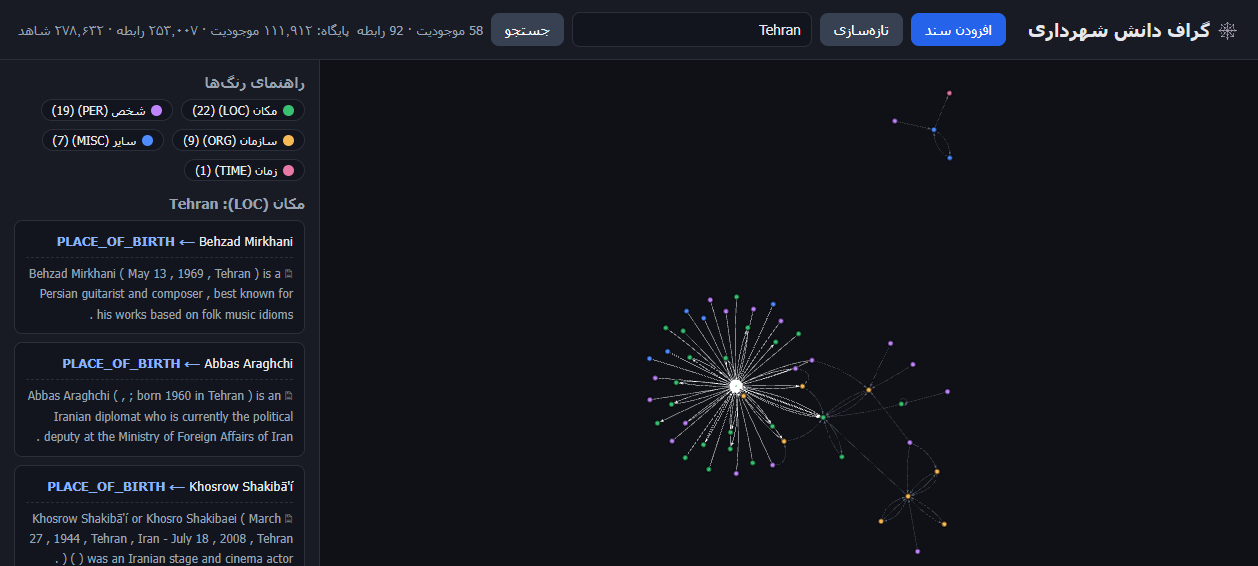
\includegraphics[width=\textwidth]{Images/graph_docred_search.png}
\caption{جست‌وجوی موجودیت در گراف $16{,}536$ سندی. سربرگ اندازه کل پایگاه و پنل کناری جمله شاهد هر رابطه را نشان می‌دهد.}
\label{fig:search}
\end{figure}

همان رابط روی خروجی \lr{Re-DocRED} هم کار می‌کند. شکل \ref{fig:neo4j} نمای مرورگر \lr{Neo4j} را بعد از بارگذاری نشان می‌دهد و شکل \ref{fig:evidence} نشان می‌دهد هر یال تا کدام جمله سند قابل ردیابی است.

\begin{figure}[ht]
\centering
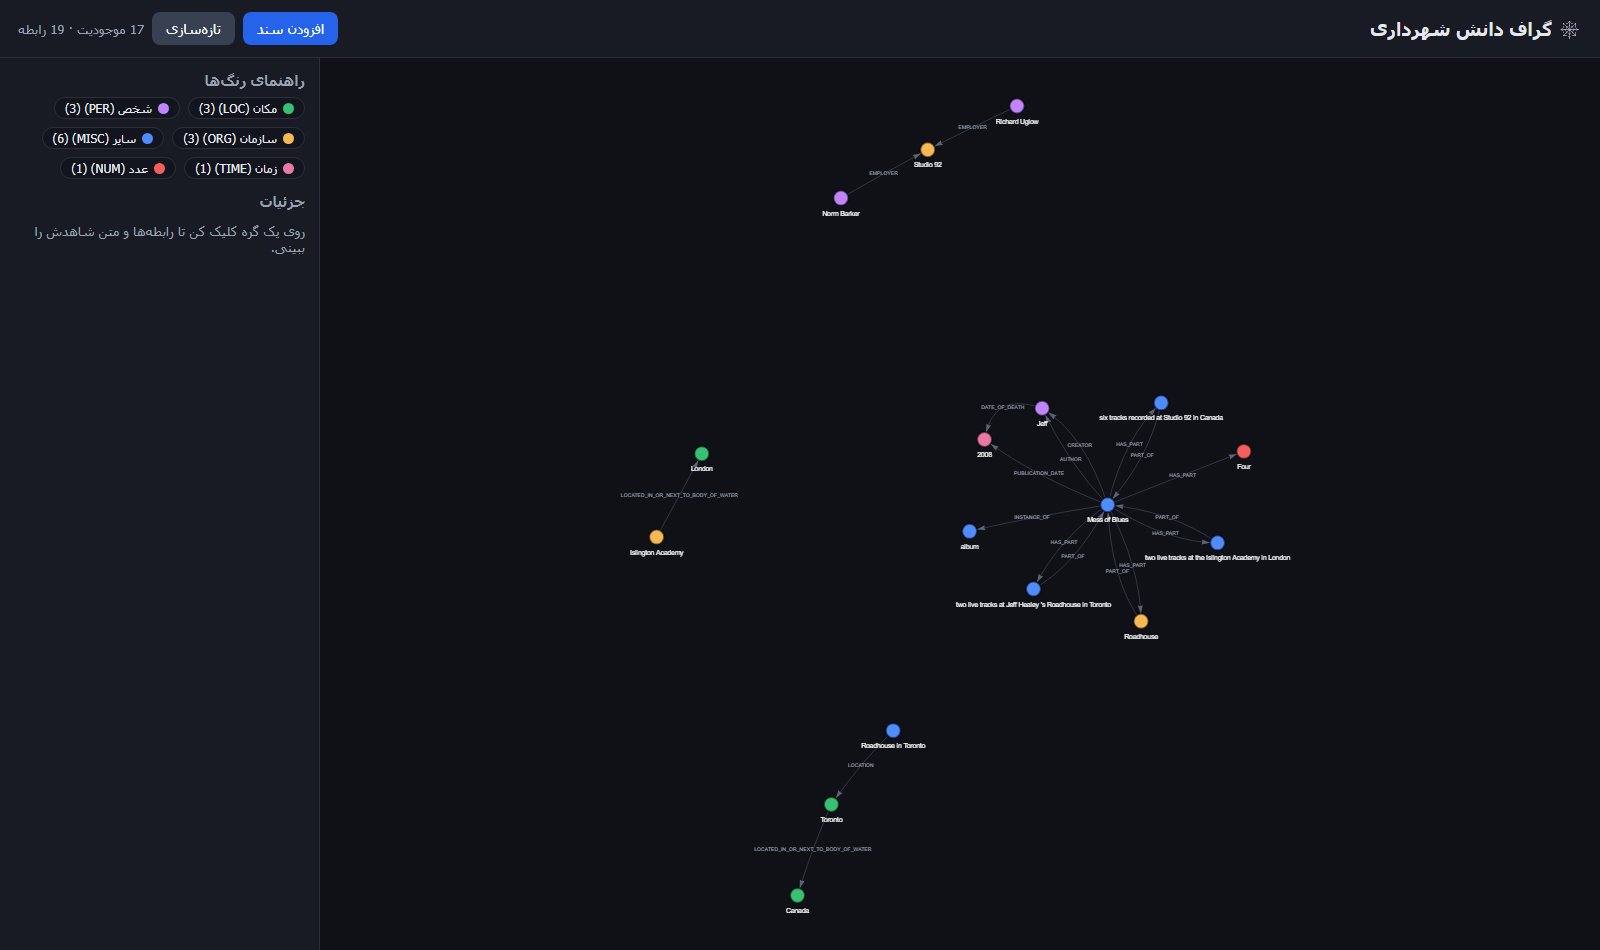
\includegraphics[width=\textwidth]{Images/graph_redocred_neo4j.png}
\caption{گراف بارگذاری‌شده در مرورگر \lr{Neo4j}. گره‌های موجودیت، یال‌های رابطه و گره‌های شاهد در یک پایگاه کنار هم می‌نشینند.}
\label{fig:neo4j}
\end{figure}

\begin{figure}[ht]
\centering
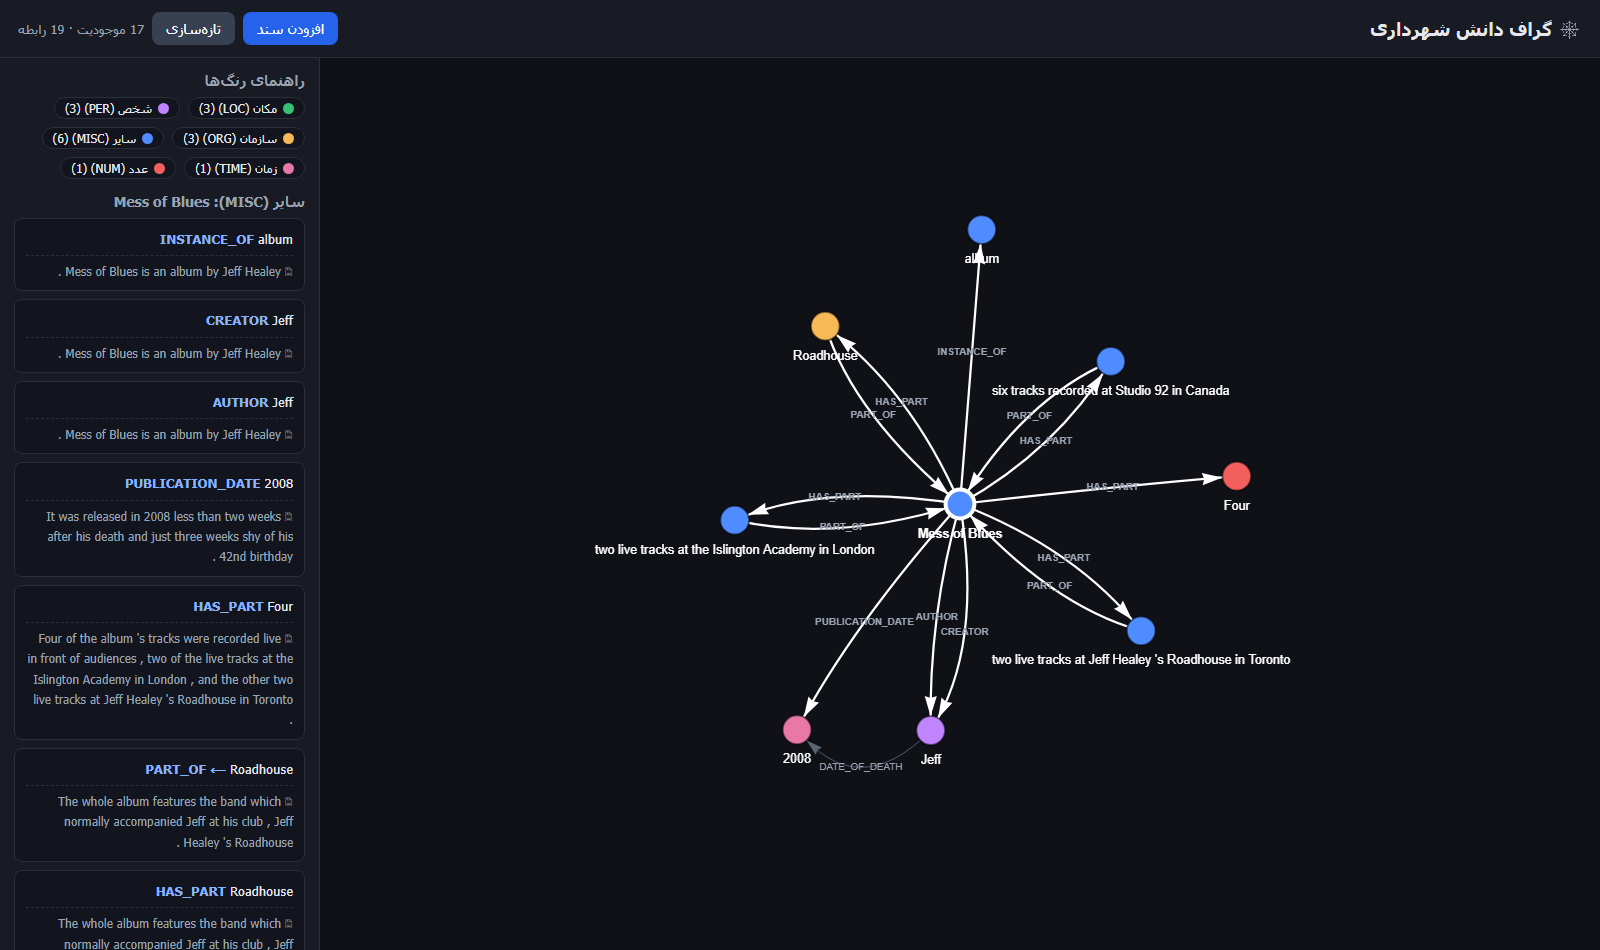
\includegraphics[width=\textwidth]{Images/graph_redocred_evidence.png}
\caption{ردیابی یک رابطه تا جمله منبع آن. هیچ یالی بدون شاهد وارد گراف نمی‌شود.}
\label{fig:evidence}
\end{figure}

\section{مقایسه با کارهای منتشرشده}
\label{sec:comparison}

جدول \ref{tab:published} کار ما را کنار نتایج منتشرشده می‌گذارد.

\begin{table}[ht]
\centering
\caption{مقایسه با کارهای منتشرشده روی \lr{Re-DocRED}.}
\label{tab:published}
\small
\begin{tabular}{|r|r|c|}
\hline
سامانه & آموزش & $F_1$ \\
\hline
\lr{KD-DocRE} \cite{kddocre} & نظارت‌شده روی $3{,}053$ سند & $81.04$ \\
\hline
\lr{ATLOP} \cite{atlop} & نظارت‌شده & $79.46$ \\
\hline
\lr{GLiDRE} \cite{glidre} & نظارت‌شده & $77.83$ \\
\hline
\lr{GPT-3.5} با \lr{NLI} \cite{gptre} & بدون آموزش و بدون مثال & $9.74$ \\
\hline
این کار (\lr{v3}) & بدون مثال، هستان‌شناسی از \lr{Train} & $23.55$ \\
\hline
این کار (\lr{v6}) & دو مثال و اجماع سه گذر & $29.66$ \\
\hline
این کار ($500$ سند \lr{Dev}) & دو مثال و اجماع دو گذر & $28.64$ \\
\hline
این کار ($500$ سند \lr{Test}) & قالب فشرده و اشتراک دو گذر & $31.70$ \\
\hline
\end{tabular}
\end{table}

حرف اصلی این جدول این است که سامانه بدون هیچ مرحله آموزش گرادیانی و فقط با دو مثال در پرامپت، بیش از سه برابر خط مبنای منتشرشده امتیاز گرفته. فاصله‌اش با مدل‌های نظارت‌شده هنوز زیاد است، ولی این فاصله را انتظار داشتیم؛ آن مدل‌ها روی سه هزار سند برچسب‌خورده آموزش دیده‌اند.

دو چیز را هنگام خواندن این جدول باید در نظر گرفت. سطر \lr{GPT-3.5} واقعاً بدون هیچ نظارتی است ولی سطرهای ما نیستند، پس مقایسه مستقیم به سود ما تمام می‌شود؛ سطر منصفانه برای چنین مقایسه‌ای \lr{v1} با $F_1$ برابر $16.88$ است. نکته دوم اینکه فقط سطر آخر روی همان بخش \lr{Test} بازبینی‌شده‌ای است که مدل‌های نظارت‌شده روی آن گزارش شده‌اند.

\section{تحلیل خطا}
\label{sec:error-analysis}

\subsection{کار مؤثر فیلتر هستان‌شناسی}
در اجرای \lr{v2} مدل زبانی $948$ سه‌تایی برگرداند و فیلتر نوع $192$ مورد، یعنی $20.3\%$، را رد کرد. پرتکرارترین ایراد چیزی بود که انتظارش را نداشتیم: معکوس بودن جهت رابطه.

\subsection{کم‌گویی، علت اصلی بازخوانی پایین}
پاسخ طلایی هر سند به‌طور میانگین $37.4$ رابطه دارد، در حالی که مدل در \lr{v1} فقط $9.3$ رابطه می‌داد و در \lr{v3} به $19.7$ رسید. الگو روشن است: مدل جمله‌های صریح را می‌بیند و از کنار حقیقت‌هایی که باید از زنجیره هم‌مرجعی یا استنتاج بیرون کشیده شوند رد می‌شود.

\subsection{نوع خطای مثبت کاذب}
از $649$ مثبت کاذب نسخه \lr{v3}، در $128$ مورد یعنی $19.7\%$ جفت‌موجودیت واقعاً رابطه دارد ولی برچسب رابطه اشتباه انتخاب شده، و در $521$ مورد یعنی $80.3\%$ جفت‌موجودیت در پاسخ طلایی هیچ رابطه‌ای ندارد. این تفکیک برایمان مهم بود، چون نوع اول با هستان‌شناسی دقیق‌تر قابل کم شدن است.

\subsection{خطای نگاشت نام}
در \lr{v6} نود سطر از $1{,}645$ سطر، یعنی $5.5\%$، به هیچ موجودیت طلایی نگاشت نشد، چون مدل نام را دقیقاً از فهرست کپی نکرده بود. همین نرخ در \lr{v3} برابر $3.6\%$ بود.

\section{ممیزی مستقل ارزیاب}
\label{sec:audit}

بعد از اینکه نتایج جمع شد، کد ارزیابی و تست‌ها را به یک مدل زبانی دیگر دادیم و از آن خواستیم علیه ادعاهای این گزارش استدلال کند. یازده ایراد گرفت که چهارتایش وارد بود و هر چهار مورد را اصلاح کردیم: کلید $\mathrm{Ign}\,F_1$ در دو بخش ناهمخوان ساخته می‌شد، تطبیق نام بیش از حد آسان‌گیر بود، گزارش خودش را «بدون نظارت» می‌نامید در حالی که هستان‌شناسی از \lr{Train} می‌آید، و سه تست ادعای نامشان را ثابت نمی‌کردند.

یک ایراد را هم رد کردیم: ادعای نشت پاسخ طلایی از لایه بستار. آن لایه فقط پیش‌بینی‌ها را می‌خواند و هیچ‌جا فایل طلایی را باز نمی‌کند. برایند این ممیزی این شد که هیچ‌کدام از اعداد $F_1$ تغییر نکرد و تنها $\mathrm{Ign}\,F_1$ حدود $0.3$ واحد جابه‌جا شد.

\chapter{مطالعه موردی فارسی}
\label{ch:casestudy}

\section{گراف دانش اسناد شهرداری}
\label{sec:municipality}

این فصل همان سامانه را بدون تغییر معماری روی داده فارسی اجرا می‌کند. چیزی که می‌خواستیم ببینیم این بود که آیا کاری که برای انگلیسی و دامنه عمومی ساخته شده، به یک زبان و دامنه دیگر منتقل می‌شود یا نه.

داده، اسناد واقع‌نمای شهرداری تهران است. آن را عمداً به‌هم‌پیوسته طراحی کردیم، یعنی یک موجودیت مثل «پروژه بهسازی پل صدر» یا یک ردیف بودجه، در چند سند مختلف و با نقش‌های متفاوت ظاهر می‌شود. جدول \ref{tab:muni} ابعادش را می‌دهد.

\begin{table}[ht]
\centering
\caption{ابعاد داده شهرداری و گراف حاصل از آن.}
\label{tab:muni}
\small
\begin{tabular}{|r|c|}
\hline
ویژگی & مقدار \\
\hline
سند منبع & $7$ \\
\hline
حجم متن خام & $811$ واژه \\
\hline
سه‌تایی خام با شاهد & $39$ \\
\hline
گره یکتا & $38$ \\
\hline
یال یکتا پس از ادغام & $32$ \\
\hline
نوع موجودیت & $6$ \\
\hline
نوع رابطه & $5$ \\
\hline
\end{tabular}
\end{table}

هستان‌شناسی این دامنه شش موجودیت دارد: پروژه، پیمانکار، مکان، مسئول، بودجه و شکایت. پنج رابطه هم میان آن‌ها تعریف شده است.

\section{نتیجه اجرا روی داده فارسی}
\label{sec:muni-result}

کل گراف را با متن منبع مقایسه کردیم و تمام رابطه‌های استخراج‌شده مورد تأیید متن بودند، یعنی چیزی نزدیک صد درصد. هیچ رابطه جعلی یا خارج از هستان‌شناسی به گراف نرسید. با کلیدگذاری بودجه بر پایه کد ثابت هم یک بودجه که در چند سند با نام‌های متفاوت آمده بود، به یک گره واحد نگاشت شد. شکل \ref{fig:muni} نمای گراف و شکل \ref{fig:muni-ev} نمونه ردیابی یک رابطه تا جمله منبع را نشان می‌دهد.

\begin{figure}[ht]
\centering
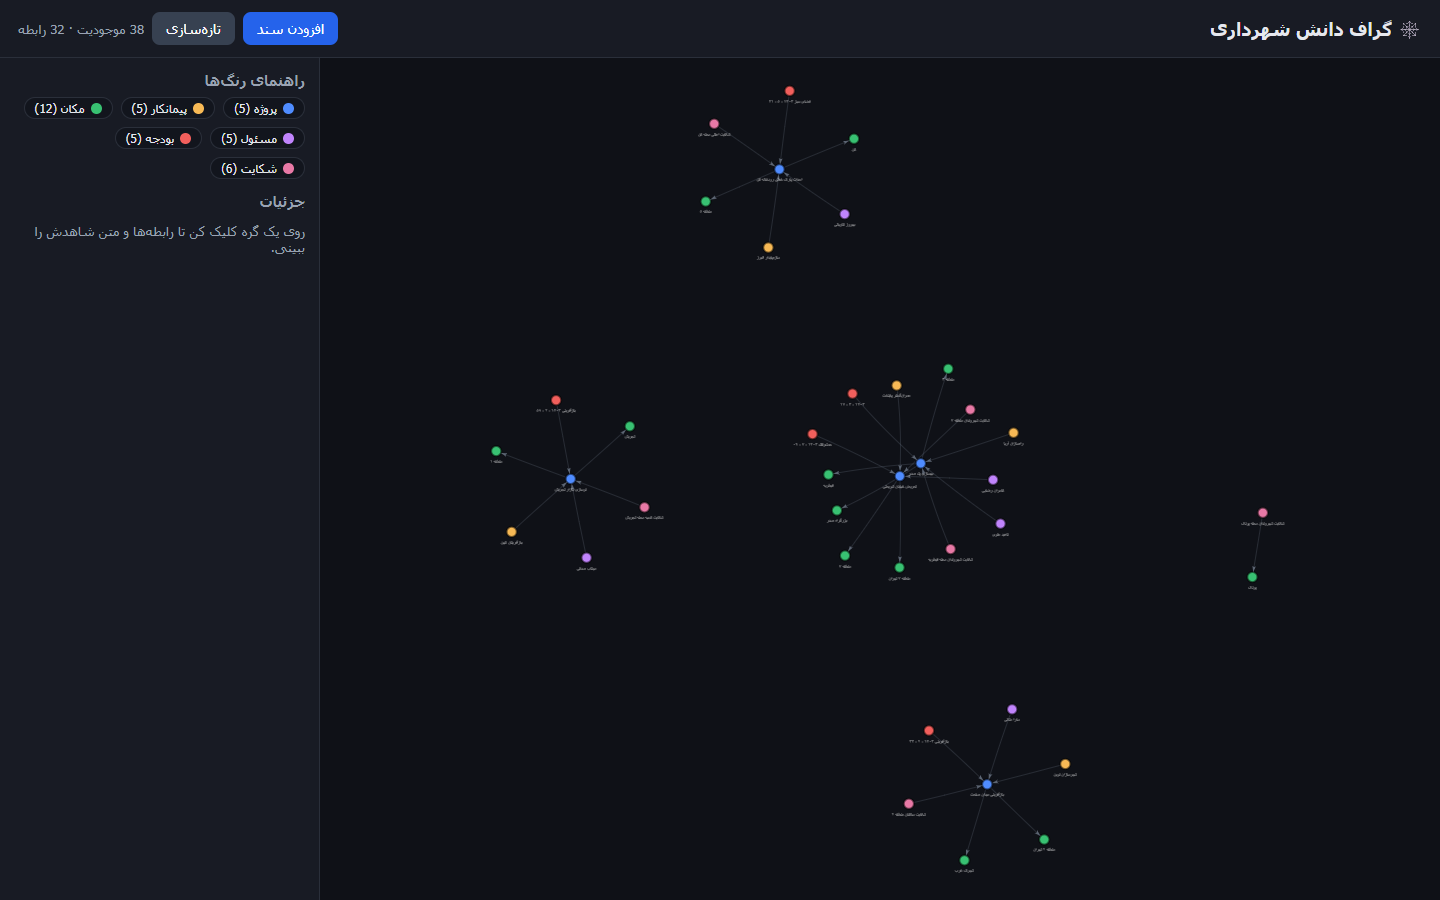
\includegraphics[width=0.9\textwidth]{Images/graph_output.png}
\caption{نمای کلی گراف دانش ساخته‌شده از هفت سند فارسی شهرداری.}
\label{fig:muni}
\end{figure}

\begin{figure}[ht]
\centering
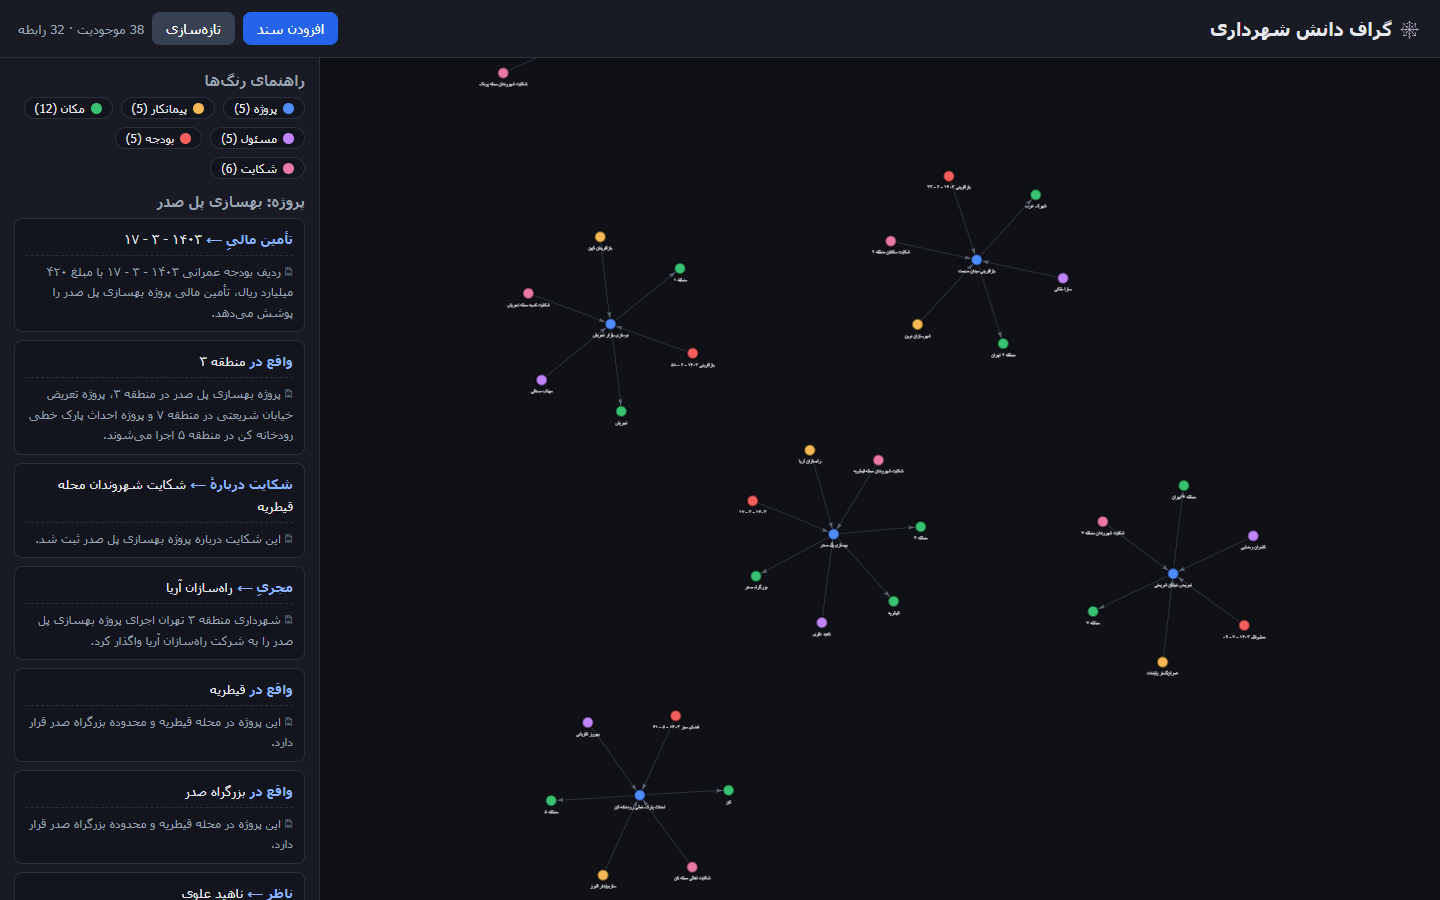
\includegraphics[width=0.9\textwidth]{Images/graph_evidence.png}
\caption{کلیک روی یک گره، رابطه‌های آن و جمله منبع هر رابطه را نشان می‌دهد.}
\label{fig:muni-ev}
\end{figure}

\section{چرا دقت اینجا صد درصد است و آنجا سی و پنج درصد}
\label{sec:why-gap}

وسوسه‌انگیز است که این تفاوت را به حساب بهتر کار کردن مدل روی فارسی بگذاریم، اما هیچ شاهدی برای چنین ادعایی نداریم. سه توضیح ساده‌تر وجود دارد.

نخست، فضای برچسب اینجا پنج رابطه دارد و آنجا نود و شش تا. وقتی مدل باید از میان پنج گزینه یکی را بردارد، احتمال انتخاب غلط طبیعتاً بسیار کمتر است.

دوم، و مهم‌تر از همه، ارزیابی اینجا دستی بود نه مبتنی بر برچسب طلایی. ما فقط می‌توانیم بگوییم هرچه استخراج شد درست بود؛ اینکه چه چیزهایی از قلم افتاد را اصلاً نمی‌دانیم. به بیان دقیق‌تر، آنچه اندازه گرفتیم دقت بود و نه بازخوانی.

سوم، اسناد شهرداری کوتاه و صریح‌اند و رابطه بین‌جمله‌ای در آن‌ها کم است، حال آنکه در \lr{Re-DocRED} بیش از نیمی از رابطه‌ها بین دو موجودیتی برقرارند که هرگز در یک جمله کنار هم نیامده‌اند.

همین مقایسه توضیح می‌دهد که چرا رفتن سراغ یک بنچمارک استاندارد ضروری بود: وقتی برچسب طلایی در کار نباشد، عدد دقت بیش از آنکه اطلاع بدهد، گمراه می‌کند.

سامانه در نهایت بدون اینکه معماری‌اش دست بخورد روی دو زبان، دو دامنه و دو هستان‌شناسی کار کرد که تعداد رابطه‌هایشان نوزده برابر با هم فرق دارد، و تنها چیزی که بین این دو اجرا عوض شد یک فایل \lr{JSON} بود. درسی که از این فصل گرفتیم این است که جدا نگه داشتن هستان‌شناسی از کد، تصمیمی که اولش فقط به چشم مرتب‌کاری می‌آمد، همان چیزی بود که انتقال‌پذیری را ممکن کرد.

\chapter{محدودیت‌ها و نتیجه‌گیری}
\label{ch:conclusion}

\section{محدودیت‌ها}
\label{sec:limitations}

\begin{enumerate}
\item برچسب بخش \lr{Test} در \lr{DocRED} عمومی نیست، پس هیچ عدد دقتی روی آن $1{,}000$ سند نداریم. نزدیک‌ترین ارزیابی بی‌طرفی که توانستیم بسازیم، بخش \lr{Train} برچسب‌خورده با $3{,}053$ سند و $F_1$ برابر $36.33$ و بخش \lr{Test} بازبینی‌شده \lr{Re-DocRED} با $500$ سند و $F_1$ برابر $31.70$ است.
\item برچسب‌های اصلی \lr{DocRED} ناقص‌اند و دقت را کمتر از واقع نشان می‌دهند؛ روی همان $498$ سند، دقت با برچسب بازبینی‌شده از $40.20$ به $66.42$ می‌رسد. برچسب بخش نظارت‌ازدور از این هم نویزی‌تر است و عددی که برایش گزارش کرده‌ایم توافق است، نه دقت.
\item نگاشت پاسخ بر پایه نام موجودیت است و نه اندیس، و همین سقفی حدود $99.7$ روی کار می‌گذارد.
\item پرامپت‌ها روی همان بخش \lr{Dev} تنظیم شدند که عدد از آن گزارش می‌شود.
\item لایه قاعده فقط سه قاعده دارد، در حالی که قاعده‌های بیشتری را می‌شود به‌صورت خودکار از بخش \lr{Train} بیرون کشید.
\item سامانه به یک مدل زبانی تجاری وابسته است، پس نتیجه به نسخه مدل هم وابسته می‌ماند.
\end{enumerate}

\section{نتیجه‌گیری}
\label{sec:conclusion}

حرف اصلی این کار یک جمله است: مدل زبانی به‌تنهایی برای ساخت گراف دانش کافی نیست. اما وقتی کنارش یک هستان‌شناسی مقیّد، الزام شاهد و یک لایه استنتاج نمادین بگذاریم، می‌شود از متن غیرساختاریافته گرافی ساخت که هم دقیق باشد و هم بتوان هر ادعایش را تا جمله منبع دنبال کرد، آن هم بدون داشتن حتی یک سند آموزشی برچسب‌خورده در آن دامنه.

روی بنچمارک استاندارد \lr{Re-DocRED}، سامانه بیش از سه برابر خط مبنای منتشرشده امتیاز گرفت: $29.66$ روی زیرمجموعه و $28.64$ روی کل $500$ سند بخش \lr{Dev}، در برابر $9.74$. در مرحله سوم، با همان معماری و تنها با سه تغییر، عدد روی $998$ سند بخش \lr{Dev} به $36.25$ رسید و روی $3{,}053$ سند بخش \lr{Train} برچسب‌خورده به $36.33$. گراف نهایی از $16{,}536$ سند ساخته شد.

چهار یافته کلیدی، که هر چهار مورد در مقیاس ده برابر هم تکرار شدند:

\begin{enumerate}
\item فیلتر هستان‌شناسی واقعاً توهم را می‌گیرد. $20.3\%$ از خروجی مدل رد شد و پرتکرارترین ایراد هم معکوس بودن جهت رابطه بود.
\item مثال کاری در پرامپت دقت را می‌خرد و نه بازخوانی را. دقت $24\%$ رشد نسبی کرد و نرخ رد شدن از $20.3\%$ به $18.7\%$ رسید.
\item گلوگاه بازخوانی است، نه دقت. مدل زبانی کم‌گوست و لایه قاعده نمادین و اجماع چند گذر با هم بازخوانی را از $10.55$ به $26.98$ رساندند.
\item مقدار $\mathrm{Ign}\,F_1$ نزدیک یا بالاتر از $F_1$ ماند، یعنی امتیاز از حفظ بودن دانش پیش‌آموخته مدل نمی‌آید و از خواندن متن سند می‌آید.
\end{enumerate}

\section{کار آینده}
\label{sec:future}

\begin{enumerate}
\item بازیابی مثال مشابه برای هر سند، به‌جای دو مثال ثابت.
\item استخراج خودکار قاعده‌های بیشتر از بخش \lr{Train}، به‌جای سه قاعده دست‌نویس.
\item رأی‌گیری وزن‌دار در اجماع با سه گذر یا بیشتر.
\item پیوند موجودیت به یک پایگاه دانش مانند \lr{Wikidata}، تا شکل‌های مختلف یک نام به یک گره برسند.
\item نگاشت بر پایه اندیس به‌جای نام، برای برداشتن سقف $99.7$.
\item افزودن لایه پرسش و پاسخ طبیعی روی گراف.
\end{enumerate}


\bibliographystyle{unsrt-fa}
\bibliography{references}
\appendix
\renewcommand{\chaptermark}[1]{\markboth{\appendixname~\thechapter: #1}{}}
\makeatletter
\bidi@patchcmd{\@makechapterhead}{\tartibi{chapter}}{\thechapter}{}{}
\makeatother
\chapter{بازتولید نتیجه}
\label{app:repro}

\section{اجرای بنچمارک}
\label{sec:app-bench}

هر عددی که در این گزارش آمده با دنباله زیر بازتولید می‌شود. مرحله آماده‌سازی، هستان‌شناسی را هم از بخش \lr{Train} می‌سازد.

\begin{latin}
\begin{verbatim}
python -m src.redocred prepare --split dev --limit 50
python -m src.redocred fewshot --n 2

python -m src.extract data/benchmark/chunks_dev.jsonl \
    --out data/benchmark/triplets_dev_v2.jsonl \
    --ontology configs/ontology_redocred.json

python -m src.extract data/benchmark/chunks_dev.jsonl \
    --out data/benchmark/triplets_dev_v4.jsonl \
    --ontology configs/ontology_redocred.json \
    --fewshot configs/fewshot_redocred.json

python -m src.redocred closure data/benchmark/_union.jsonl \
    --out data/benchmark/triplets_dev_v6.jsonl

python -m src.redocred eval data/benchmark/triplets_dev_v6.jsonl \
    --gold data/benchmark/gold_dev50.jsonl \
    --report data/benchmark/eval_report_v6.json
\end{verbatim}
\end{latin}

\section{اجرای پیکره کامل}
\label{sec:app-full}

\begin{latin}
\begin{verbatim}
python -m src.docred prepare
python -m src.docred stats

python -m src.extract data/benchmark/docred/chunks_validation.jsonl \
    --out data/benchmark/docred/triplets_validation_a.jsonl \
    --ontology configs/ontology_redocred.json --compact --workers 16

python -m src.redocred consensus <pass A> <pass B> --out <agreed>
python -m src.redocred closure  <agreed>  --out <final>

python -m src.load_neo4j data/benchmark/docred/triplets_validation.jsonl \
    --ontology configs/ontology_redocred.json
\end{verbatim}
\end{latin}

هر دو گذر ازسرگیری‌پذیرند. اگر اجرا نیمه‌کاره بماند، همان فرمان کار را از همان‌جا ادامه می‌دهد، چون خروجی در یک فایل کناری نوشته می‌شود و اجرای بعدی آن را هم می‌خواند.

\section{تست‌های آفلاین}
\label{sec:app-tests}

دوازده تست بدون شبکه و بدون فراخوانی مدل زبانی اجرا می‌شوند:

\begin{latin}
\begin{verbatim}
python -m tests.test_extract
python -m tests.test_redocred
\end{verbatim}
\end{latin}

خروجی هر دو باید \lr{all passed} باشد.

\chapter{فایل‌های تولیدشده}
\label{app:files}

\begin{table}[ht]
\centering
\caption{فایل‌های اصلی سامانه و کاری که هر کدام انجام می‌دهند.}
\label{tab:files}
\begin{adjustbox}{max width=\textwidth}
\small
\begin{tabular}{|p{5cm}|p{8.8cm}|}
\hline
\rg فایل & \rg محتوا \\
\hline
\rg \lr{src/ingest.py} & \rg ورود سند، رونویسی تصویر، نرمال‌سازی، قطعه‌بندی \\
\hline
\rg \lr{src/extract.py} & \rg استخراج با مدل زبانی، اعتبارسنجی، فیلتر هستان‌شناسی، قالب فشرده \\
\hline
\rg \lr{src/redocred.py} & \rg آماده‌سازی بنچمارک، ساخت مثال، اجماع، بستار، ارزیاب \\
\hline
\rg \lr{src/docred.py} & \rg خواندن چهار بخش \lr{Parquet} پیکره \lr{DocRED} و ساخت داده و آمار \\
\hline
\rg \lr{src/load\_neo4j.py} & \rg بارگذاری تکرارپذیر در \lr{Neo4j} \\
\hline
\rg \lr{src/app.py} & \rg رابط وب نمایش و جست‌وجوی گراف \\
\hline
\rg \lr{configs/ontology\_redocred.json} & \rg $96$ رابطه و $654$ ترکیب مجاز \\
\hline
\rg \lr{configs/fewshot\_redocred.json} & \rg مثال‌های پرامپت، برگرفته از بخش \lr{Train} \\
\hline
\rg \lr{data/benchmark/docred/claude/} & \rg خروجی و گزارش عددی هر بخش در مرحله سوم \\
\hline
\end{tabular}
\end{adjustbox}
\end{table}


%کلمات کلیدی انگلیسی
\latinkeywords{knowledge graph, document-level relation extraction, large language models, constrained ontology, hallucination control, DocRED}
%چکیده انگلیسی

\en-abstract{
Most of what an organisation knows sits in free text, where no query can reach it. This work builds a system that extracts (entity, relation, entity) triples from unstructured text and loads them into a queryable knowledge graph. Three decisions separate it from a plain call to a language model: a constrained ontology that rejects every triple whose (subject type, relation, object type) combination is not allowed, a mandatory evidence rule that ties each edge to the sentence it came from, and a pipeline that never duplicates data when it runs again.
\\
The system was evaluated on the Re-DocRED benchmark. Over six iterations $F_1$ rose from 16.88 to 29.66, against a published GPT-3.5 baseline of 9.74 on the same data. The same configuration then scored 28.64 on all 500 documents of the dev split. Stage three moved to the full DocRED corpus, 106,924 documents and 1.56 million labelled triples, which forced a rewrite for scale: concurrent extraction, resumption without repeated work, a streaming evaluator and a batched Neo4j loader.
\\
Changing the language model, compacting the answer format and taking the intersection of two passes instead of their union raised $F_1$ to 36.25 on the 998 dev documents and to 36.33 on the 3,053 annotated train documents, which played no part in prompt tuning. A fixed prediction set scored against two label sets on the same 498 documents gives precision 40.20 with the original labels and 66.42 with the revised ones, which measures the false negative problem in DocRED directly. The final graph, built from 16,536 documents, holds 111,912 entities, 253,007 relations and 278,632 evidence nodes. The same system, with no architectural change, then ran on Persian municipal documents: only one ontology file was different.
}
%%%%%%%%%%%%%%%%%%%%% کدهای زیر را تغییر ندهید.

\newpage
\thispagestyle{empty}
\begin{latin}
\section*{\LARGE\centering Abstract}

\een-abstract

\vspace*{.5cm}
{\large\textbf{Key Words:}}\par
\vspace*{.5cm}
\elatinkeywords
\end{latin}

\baselineskip=.6cm
\begin{latin}

\latinfaculty{Department of Math and Computer Science}

\latintitle{Automatic Knowledge Graph Construction from Unstructured Text with Large Language Models}

\firstlatinsupervisor{Dr. Mehdi Ghatee}

\secondlatinsupervisor{Dr. Behnam Yosefimehr}

\latinname{Mostafa}

\latinsurname{Rastegar}

\latinthesisdate{September 2026}

\latinvtitle
\end{latin}

\end{document}
